\chapter{Bluetooth Stack Implementation}
\label{chp:btstackimp}
\lhead{Chapter \ref{chp:btstackimp}. \emph{Bluetooth Stack Implementation}}

The development of the Bluetooth stack followed a bottom-up development methodology, designing and writing each software layer in sequence from the lowest layer first, to the highest and most abstracted layers last. This sequence ensured that each layer was functionally correct and could be verified before the higher layers were implemented. This suited the development of the Bluetooth stack---and, indeed, most software stacks---as each higher software layer is dependant solely on lower logical layers in the stack.

\section{Software Overview}

The software layers implemented in the completed Bluetooth stack are shown in Figure \ref{fig:completedbtstacklayers}.

\begin{figure}[tbph]
	\vspace{1em}
	\centering
		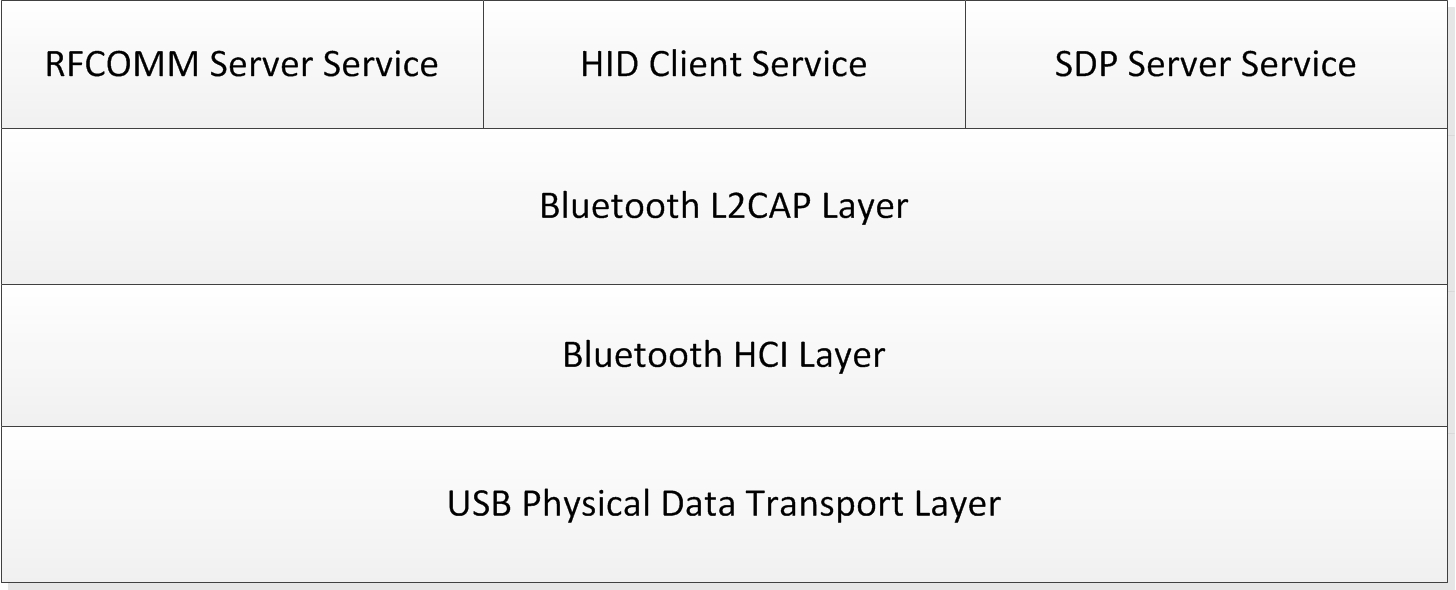
\includegraphics[width=100mm]{CompletedBluetoothStack.png}
	\rule{35em}{0.5pt}
	\caption[Diagram of the completed Bluetooth stack layers]{Diagram showing the completed layers of the Bluetooth stack.}
	\label{fig:completedbtstacklayers}
\end{figure}

Each software layer was implemented as a seperate pair of source code module files, written in the C language and targeted towards the C99 language specification. Configuration for the stack is located in the file \texttt{BluetoothCommon.h}, which must be included in the user application to operate the stack.

% TODO

\section{Design Restrictions}

A number of design restrictions were placed on the development of the Bluetooth stack; these ensured that the completed stack remained modular, extensible and suitable for integration in a wide range of embedded systems with various capabilities, and conversely, limitations. As an unfortunate but expected side effect, a number of these restrictions complicated the software development process significantly.

\FloatBarrier
\subsection{No Heap Memory Allocations}

The largest restriction placed on the stack design was the requirement of static and stack allocated memory allocation only --- no dynamic heap allocated memory was to be used via the usual \lstinline{malloc()} and \lstinline{free()} functions from the \texttt{libc} library. Most embedded environments contain three types of memory allocations:

\begin{enumerate}
	\item \textbf{Static Allocations}, including global variables and \lstinline{static} qualified variables.
	\item \textbf{Stack Allocations}, automatically populated to store local automatic variables, function paramaters, return addresses, etc.
	\item \textbf{Heap Allocations}, persistant dynamic allocations manually managed by the user application.
\end{enumerate}

However, for significantly memory constrained systems, heap allocations are generally avoided due to the possibility of memory fragmentation; large numbers of differently-sized allocations and deallocations may cause fragmented holes to appear within the heap environment, causing allocation exhaustion to occur even if sufficient (raw) memory is available for an allocation request. In addition, dynamic memory complicates the formal analysis of a program, making memory requirements harder to judge, and thus harder to determine whether a given set of firmware will operate correctly within a specified environment without further in-depth analysis. In large embedded environments (ones with virtual memory management, and/or a large heap space) these problems are less of an issue and dynamic memory may be preferable for its simplicity.

The design of embedded stacks based on a no-heap-allocation strategy is a complex one, requiring certain trade-offs to be made. In the case of the Bluetooth stack presented here, a major side-effect of this decision was the need to fix the maximum number of simultaneous HCI device connections, L2CAP channel connections, and other queue- and list-like data structures within each instance of the stack. A major downside to this approach is the increased complexity of packet buffering and re-assembly, as fixed-size buffers must be used.

\FloatBarrier
\subsection{Endianness Correction}

A second complication based on the physical constraints from the execution environment is the native endianness of the processor hardware, i.e., the order in which multiple-byte data values are stored inside the processor. Depending on the execution architecture, data values may be represented in Big Endian (most significant byte at the lowest address) or Little Endian (least significant byte at the lowest address) format within the CPU. Data transmitted and received at the local device to remote device boundary must undergo a encoding conversion if the endianness of the source and sink do not match.

In the case of the Bluetooth specification, this was further complicated by the various layers; some layers used Little Endian encoding for exchanged data, while others selected Big Endian. To perform the correct encoding/decoding on each platform, a set of conversion macros were implemented at points where multi-byte values were exchanged. This ensured that regardless of the native endian format of the architecture the stack is compiled to, multi-byte values will be interpreted correctly.

\FloatBarrier
\subsection{Physical Transport Independance}

As the Bluetooth 2.1 specification outlines a several possible physical transports of HCI packets between the Bluetooth transceiver silicon and the application microcontroller, it was important that the physical transport layer be made independant from the rest of the stack. By making no assumptions about the form of transport protocol used to transfer packets to and from the attached Bluetooth silicon, the user application is free to implement their own transport mechanism without having to modify the internals of the stack. One instance of the stack may run across a USB connection to an attached Bluetooth module, while another may simultaneously connect to the microcontroller over a USART link.

\FloatBarrier
\subsection{Bluetooth Specification Compatibility}

For a software stack to be suitable for general use, it must be designed around, and undergo a series of tests to ensure compatibility with, a particular version of the protocol specification. Without a fixed version of a specification, correctness of the finished stack and compatibility with other implementations of the same technology cannot be assured.

As a \textit{compliant} stack would require extensive development and expensive certification procedures, the stack was instead aimed to be \textit{compatible} with version 2.1 of the Bluetooth specification. This subtle difference in the terminology indicates a large difference in the restrictions around the exact implementation. While a \textit{compliant} stack must be verified against the entire specification and rigorously tested to ensure exact conformance, a \textit{compatible} must only work with (most) other devices implementing their own compliant or compatible stacks of the same protocol version.

In the future the stack could be made conformant if desired, however for the purposes of the project only protocol compatibility was tested.

\FloatBarrier
\subsection{Multiple Stack Instances}

For maximum utility, the stack was designed to allow for multiple simultaneous stack instances. This was implemented to allow for unusual Bluetooth usage scenarios where more than one tranceiver is desirable in the one system, either for security, wireless signal coverage or bandwidth reasons. Each physical transceiver is allocated a logical stack instance, capable of sustaining one or more simultaneous connections, and one or more logical channels between devices. This flexibility ensures that the majority of usage scenarios are covered by the stack's implementation.

Code-wise, the multiple stack functionality is implemented as a common first parameter to all functions within the stack, \lstinline{BT_StackConfig_t* const StackState}. This parameter is used to pass around a reference to the stack instance being operated upon, and is somewhat analagous to the \lstinline{this} property in C++ classes, if the entire stack was wrapped in a single class. As the stack was written in the C language which lacks Object Orientated language capabilities, this form of basic polymorphism was implemented manually. For each physical tranceiver, the user application is expected to declare a new instance of the \lstinline{BT_StackConfig_t} structure within their code, and pass this to the main Bluetooth stack management routines (see Listing \ref{lst:stackconfig}).

\lstinputlisting[float=tbph,caption={Configuration example of a Bluetooth stack instance.},label={lst:stackconfig}]{./Figures/StackConfig.c}

\FloatBarrier
\subsection{Multiple Simultaneous Connections and Channels}

The HCI connections and L2CAP channels for each stack instance are implemented as an pair of object pools within the \lstinline{BT_StackConfig_t} structure; L2CAP channel objects within the pool are shared amongst all established HCI connections --- for example, one HCI connection may use all the available L2CAP channels, or two connections may share the pool equally. This design decision allows the full pool of L2CAP channel objects to be used by the stack regardless of the HCI connection requesting them. Figure \ref{fig:stackobjectpools} illustrates a single stack instance with a typical usage scenario, with two of the stack's HCI objects containing established connections, each with several L2CAP channel objects associated with the connection from the channel object pool.

\begin{figure}[tbph]
	\vspace{1em}
	\centering
		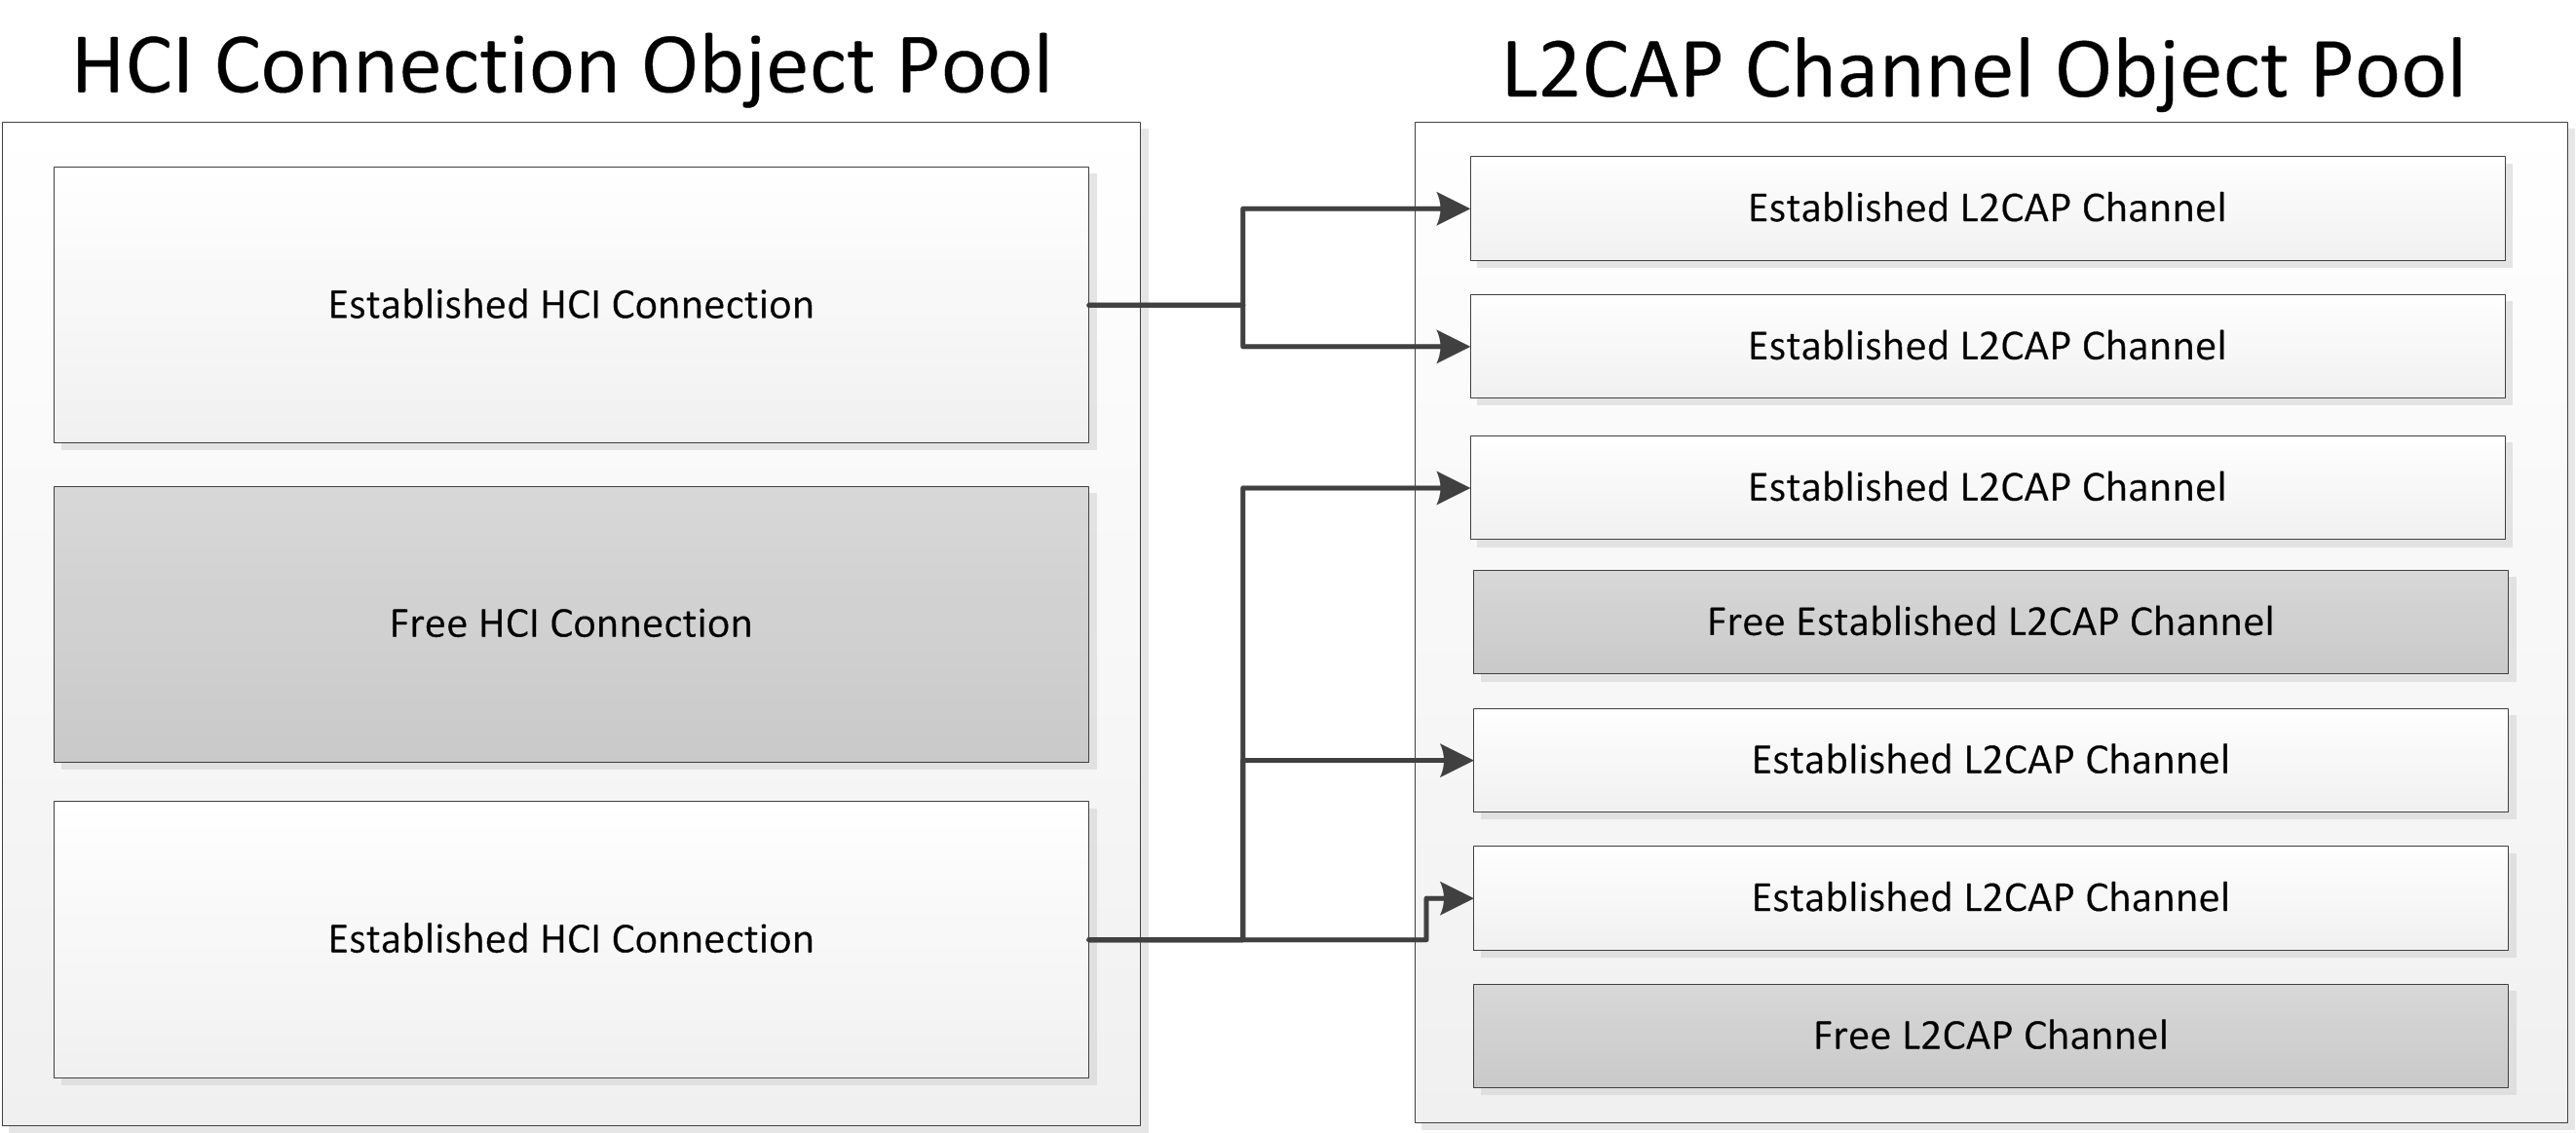
\includegraphics[width=140mm]{StackObjectPools.png}
	\rule{35em}{0.5pt}
	\caption[Diagram of the Bluetooth stack instance object pools]{Diagram showing the HCI Connection and L2CAP object pools within a stack instance.}
	\label{fig:stackobjectpools}
\end{figure}

To positively link one used L2CAP channel instance to its parent HCI connection object, the HCI connection's \texttt{handle} property is stored in the L2CAP channel object as a primary key. This handle value, allocated uniquely by the external Bluetooth HCI controller silicon when a new HCI connection is made, is then used to locate the HCI connection object within a stack instance from an established channel instance. While a pointer to the parent HCI object would offer a faster method of locating the associated HCI connection, this would tightly couple the HCI layer with the L2CAP layer as the former would need to alter the latter's objects if and when HCI connections are terminated.

As the stack does not use heap-based dynamic memory allocation, this approach ensures that the stack contains similar levels of flexability to a dynamically allocated object approach, with only a minimal overhead. The maximum size of each object pool is set via the Bluetooth Stack's \lstinline{BT_MAX_DEVICE_CONNECTIONS} and \lstinline{BT_MAX_LOGICAL_CHANNELS} configuration defines.

\FloatBarrier
\subsection{Minimal Memory Usage}

While large embedded systems may run the completed Bluetooth stack, the design decisions made during its development were primarily aimed at ensuring the best performance and smallest footprint in very low powered microcontrollers. This resulted in the stack being optimised for small systems; only the minimal attributes required to establish and maintain connections are stored by the stack. One example of these optimizations is in the event system (described in detail later in this chapter) implementation: rather than implementing a callback registration system for each event, named callbacks are used instead. Various portions of the Bluetooth stack expect the user application to provide callback and event functions using names and prototypes defined in the stack header files.

This named callback function system reduces the memory footprint of the stack, as the callback addresses do not need to be stored in RAM at runtime, and the compiler does not need to inflate the binary with additional functions to manage the callback function registrations.

\section{Software Layer Implementation}

% TODO

\FloatBarrier
\subsection{Physical Transport}

% TODO

\FloatBarrier
\subsection{HCI Layer}

% TODO

\FloatBarrier
\subsection{L2CAP Layer}

% TODO

\FloatBarrier
\subsection{Bluetooth Services}

% TODO

\FloatBarrier
\subsubsection{SDP Service}

% TODO

\FloatBarrier
\subsubsection{HID Service}

% TODO

\FloatBarrier
\subsubsection{RFCOMM Service}

% TODO

\section{Integration into User Applications}

% TODO

\FloatBarrier
\subsection{Events and Callbacks}

\begin{figure}[tbph]
	\vspace{1em}
	\centering
		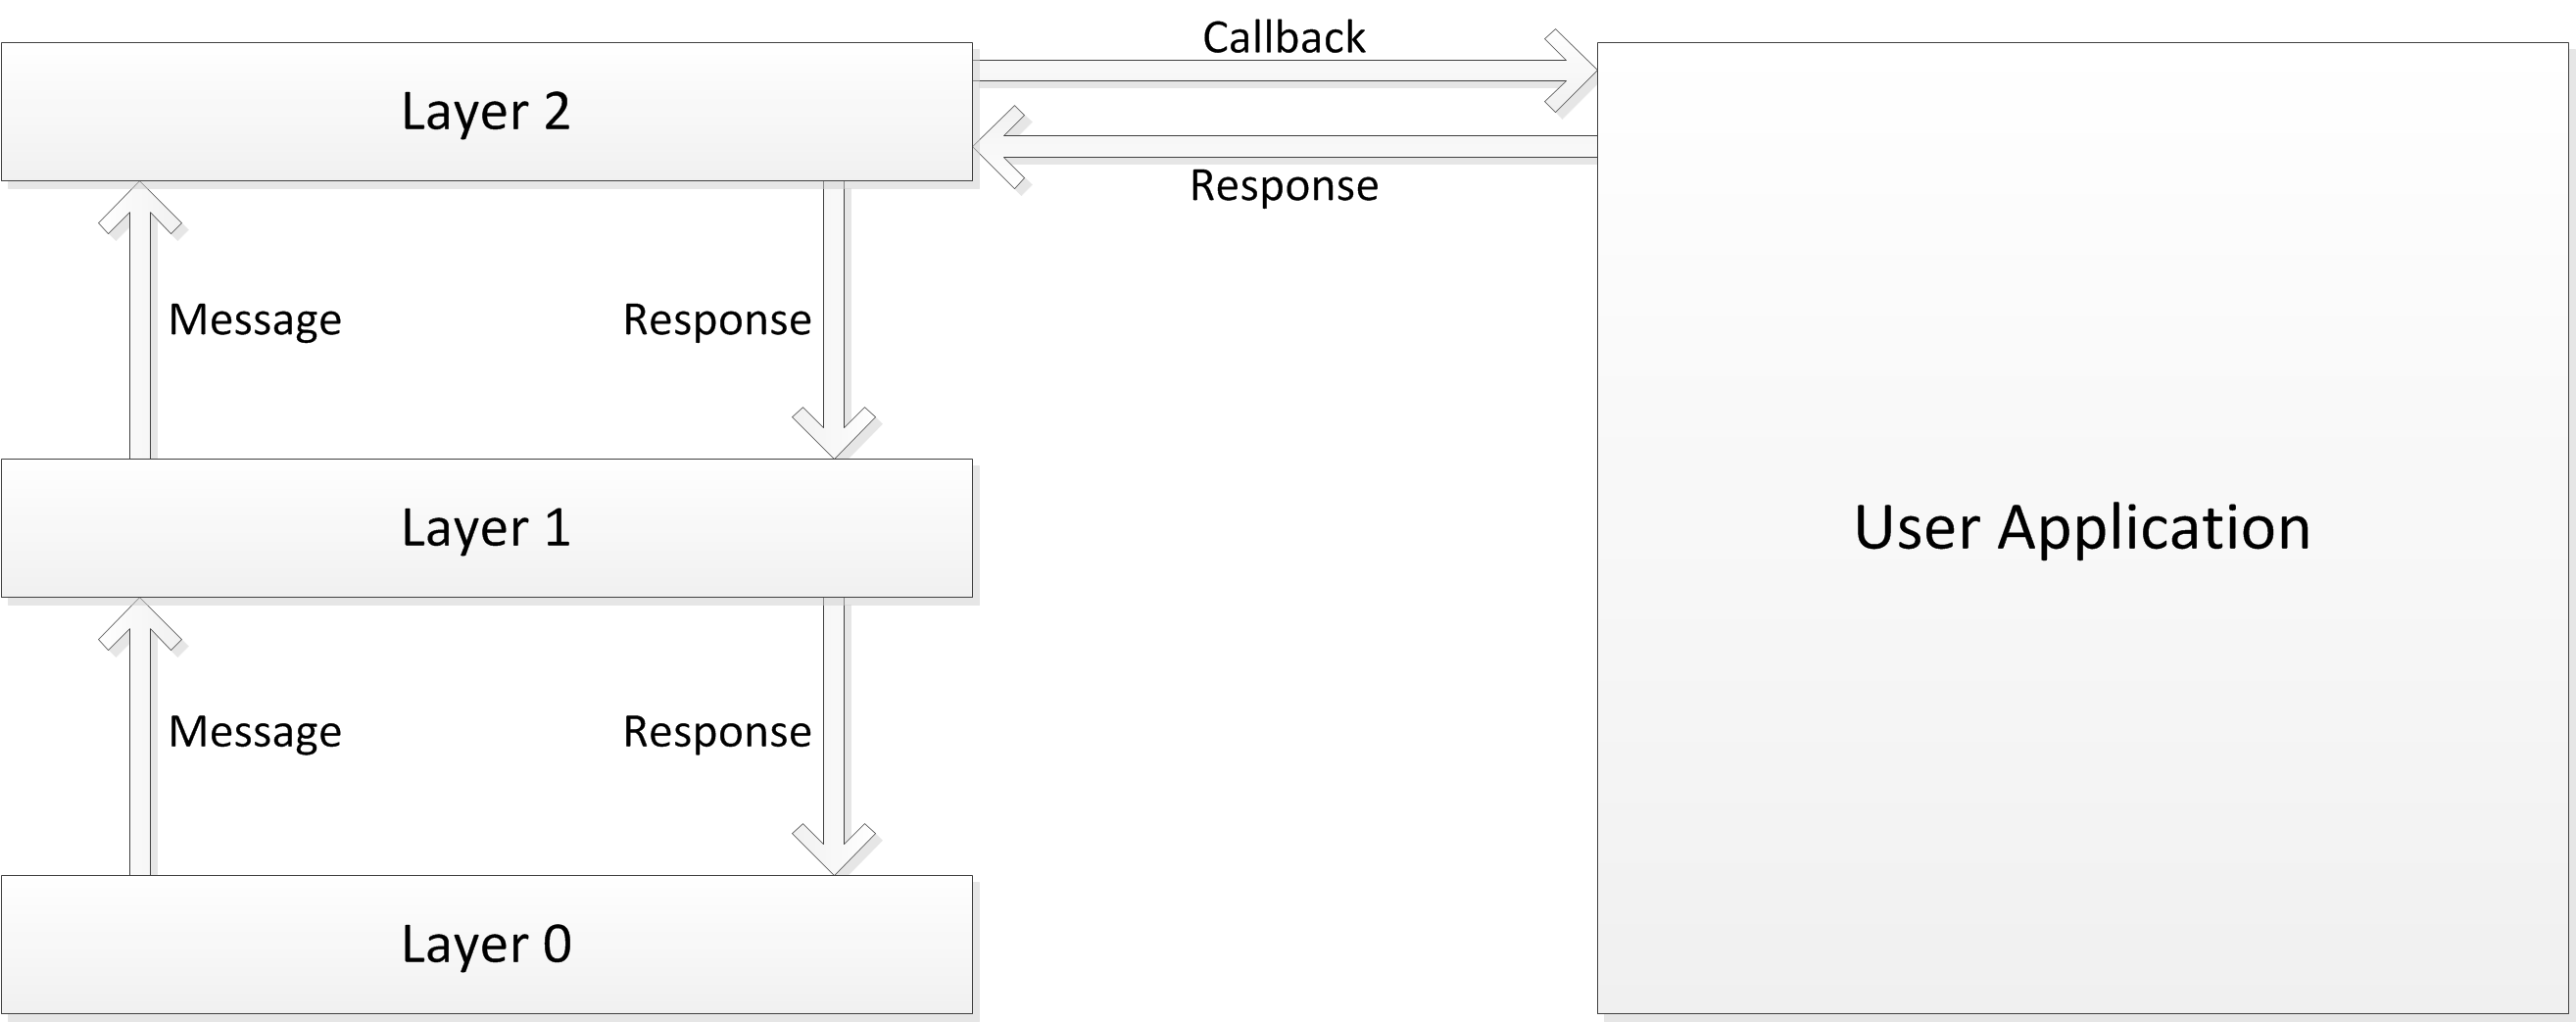
\includegraphics[width=140mm]{MessageResponseCallback.png}
	\rule{35em}{0.5pt}
	\caption[Diagram of the Message, Response and Callback sequence]{Diagram showing the Message, Response and Callback sequence of a typical software stack when passing a message and response through several intermediate layers.}
	\label{fig:messageresponsecallback}
\end{figure}

% TODO

\FloatBarrier
\subsection{Management Functions}

% TODO